\documentclass[10pt,a4paper]{article}
%\usepackage[english,spanish]{babel}
\usepackage{indentfirst}
\usepackage{anysize} % Soporte para el comando \marginsize
%\marginsize{1.5cm}{1.5cm}{0.5cm}{1cm}
\marginsize{2,5cm}{1,8cm}{4cm}{1,7cm}
\usepackage[psamsfonts]{amssymb}
\usepackage{amssymb}
\usepackage{amsfonts}
\usepackage{amsmath}
\usepackage{amsthm}
\usepackage{stackrel}
\usepackage{graphicx}
\usepackage[colorinlistoftodos]{todonotes}
%Color a las referencias
\usepackage[colorlinks=true, allcolors=blue]{hyperref}
\usepackage[spanish]{babel}
\selectlanguage{spanish}
\usepackage[utf8]{inputenc} 

\usepackage{multicol}
\renewcommand{\thepage}{}
\columnsep=7mm

%%%%%%%%%%%%%%%%%%%%%%%%%%%%%%%%%%%%%%%%
\newtheorem{definicion}{Definici\'on}[section]
\newtheorem{teorema}{Teorema}[section]
\newtheorem{prueba}{Prueba}[section]
\newtheorem{prueba*}{Prueba}[section]
\newtheorem{corolario}{Corolario}[section]
\newtheorem{observacion}{Observaci\'on}[section]
\newtheorem{lema}{Lema}[section]
\newtheorem{ejemplo}{Ejemplo}[section]
\newtheorem{solucion*}{Soluci\'on}[section]
\newtheorem{algoritmo}{Algoritmo}[section]
\newtheorem{proposicion}{Proposici\'on}[section]

\linespread{1.4} \sloppy

\newcommand{\R}{\mathbf{R}}
\newcommand{\N}{\mathbf{N}}
\newcommand{\C}{\mathbb{C}}
\newcommand{\Lr}{\mathcal{L}}
\newcommand{\fc}{\displaystyle\frac}
\newcommand{\ds}{\displaystyle}

\DeclareMathOperator{\Dom}{Dom}

%%%%%%%%%%%%%%%%%%%%%%%%%%%%%%%%%%%%%%%%

\renewcommand{\thefootnote}{\fnsymbol{footnote}}
\usepackage{url}
\usepackage{hyperref}

\begin{document}
\begin{center}
 {\Large \textbf{MODELAMIENTO DE LA ECONOMÍA DE UN PAÍS}}
\end{center}
\begin{center}
 Gustavo Lozano$^{1}$, Miller Silva$^{2}$, Victor Ponce$^{3}$, Nicks Lazaro$^{4}$, Kevin Solano$^{5}$ \vskip5pt
 {\it Facultad de Ciencias$^1$, Universidad Nacional de Ingenier\'{\i}a$^1$\\}\vskip5pt
 Email: glozanoa@uni.pe$^{1}$, miller.silva.m@uni.pe$^{2}$, victor.ponce.p@uni.pe$^{3}$, elazaroc@uni.pe$^{4}$
\end{center}
%\maketitle 
\vspace*{1cm}
\begin{abstract}

\noindent Las matemáticas son de gran importancia y ayuda para el progreso de muchas disciplinas, como por ejemplo la economía. El desarrollo de este método combina el uso de la teoría económica, el análisis estadístico y matemático. Introducir ciertas simplificaciones y supuestos para crear un modelo que ayudara a predecir los niveles de producción futuros de cada sector o industria, a fin de satisfacer las demandas futuras para diversos productos. La actividad económica en la región se divide en un número de segmentos o de sectores productivos. Cada sector agrupa actividades que tienen diferentes ritmos de consumo y producción de bienes. Parte de la producción de un sector (Output) puede ir al consumo (Input) de otro distinto sector. Esta información se recolecta en forma de una matriz. Los paises poseen muchas industrias relevantes causando que se generan matrices muy grandes, encontrar la solucion manualmente es muy ineficiente, por ello recurimos al uso de computadores. Para poder confiar en los resultados de la maquina hacemos uso del \textbf{análisis numérico} encontrando los metodos adecuados para obtener la solución con menor error.

\end{abstract}

\begin{quotation}
	{\small
		\noindent\textbf{Palabras Clave:} \\ 
	Análisis estadístico, Demanda futura, Sector industrial, Producción futura, Análisis numérico\\
	}
\end{quotation}

\renewcommand{\abstractname}{Abstract}
\begin{abstract}
	\noindent Mathematics is of great importance and helps the progress of many disciplines, such as economics. The development of this method combines the use of economic theory, statistical and mathematical analysis. Economic activity in the region is divided into a number of segments or productive sectors. Each sector groups activities that have different rates of consumption and production of goods. Part of the production of a sector (Output) can go to the consumption (Input) of another different sector. This information is collected in the form of a matrix. Countries have a large number of industries, which generates very large matrices, finding the solution manually is very inefficient, therefore, we resort to the use of computers. To be able to trust the results of the machine, we make use of the \textbf{Numerical Analysis} finding the adequate methods to obtain the solution with less error.
	
\end{abstract}


\begin{quotation}
	{\small
		\noindent \textbf{Keywords:} \\ 
		Statistical analysis, Future demand, Industrial sector, Future production, Numerical analysis\\
	}
\end{quotation}


\pagebreak

\begin{multicols}{2}
\begin{center}
{\large \bf 1. INTRODUCCI\'ON}
\end{center}
 Con el fin de comprender y ser capaz de manipular la economía de un país o una región, uno tiene que llegar a un cierto modelo basado en los diversos sectores de esta economía. El modelo de Leontief es un intento en esta dirección. Basado en la suposición de que cada industria en la economía tiene dos tipos de exigencias: la demanda externa (de fuera del sistema) y la demanda interna (demanda de una industria por otro en el mismo sistema), el modelo de Leontief representa la economía como un sistema de ecuaciones lineales. El modelo de Leontief fue inventado en los años 30 por el profesor Wassily Leontief \color{blue} Fig 1 \color{black} que desarrolló un modelo económico de la economía de Estados Unidos mediante su división en 500 sectores económicos. El 18 de octubre de 1973, el profesor Leontief fue galardonado con el Premio Nobel de economía por su esfuerzo.\\
 
\begin{center}
	\centering
	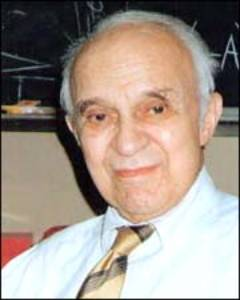
\includegraphics[width=5cm,height=5cm]{leontief.jpg}
	\\
	Fig1: Profesor Wassily Leontief
\end{center}

\begin{center}
{\large \bf 2. CONCEPTOS PREVIOS}
\end{center}
Hay dos tipos de modelados de la economía que estableció Leontief: el modelo cerrado y el modelo abierto.\\
\begin{itemize}
	\item \textbf{EL MODELO CERRADO DE LEONTIEF} : Considerar una economía que consiste en $n$ industrias (o sectores)   $S_{1}, ... , S_{n}$. Eso significa que cada industria consume algunos de los bienes producidos por las otras industrias, incluso a sí misma (por ejemplo, una planta generadora de energía utiliza parte de su propia energía para la producción). Decimos que tal economía esta cerrada si satisface sus propias necesidades. Es decir, no hay mercancías que salgan o entren en el sistema. Sea $m_{ij}$ el número de unidades producidas por la industria $S_{i}$ y necesarias para producir una unidad de la industria $S_{j}$. Si $p_{k}$ es el nivel de producción de la industria $S_{k}$, luego $m_{ij}p_{j}$ representa el número de unidades producidas por la industria $S_{i}$ y consumidas por la industria $S_{j}$. Entonces, el número total de unidades producidas por la industria $S_{i}$ viene dado por:
	$$ m_{i1}p_{1} + m_{i2}p_{2} + ... + m_{in}p_{n} $$
Para tener una economía equilibrada, la producción total de cada industria debe ser igual a su consumo total. Esto nos dará el siguiente sistema lineal:
\begin{equation*}
	\begin{matrix}
	m_{11}p_{1} &+& m_{12}p_{2} &+& \ldots  &+ &m_{1n}p_{n} &=& p_{1}\\
	m_{21}p_{1} &+& m_{22}p_{2} &+&\ldots  &+& m_{2n}p_{n} &=& p_{2}\\
	\vdots&&\vdots&&&&\vdots&&\vdots\\         
	m_{n1}p_{1} &+& m_{n2}p_{2} &+& ... & +& m_{nn}p_{n} &=& p_{n}
	\end{matrix}
\end{equation*}\\
Luego, la matriz $A$ es:   
    
 \[ A =
 \left( \begin{array}{cccc}
 m_{11} & m_{12} & \cdots & m_{1n} \\ 
 m_{21} & m_{22} & \cdots & m_{2n} \\
 \vdots & \vdots & \ddots & \vdots \\
 m_{n1} & m_{n2} & \cdots & m_{nn}
 \end{array} \right) \]\\
 
Entonces nuestro sistema a resolver se puede escribir como $AP = P$, donde:
	
 \[ P =
\left( \begin{array}{cccc}
p_{1} \\ 
p_{2} \\ 
\vdots  \\
p_{n} \\ 
\end{array} \right) \]\\
 $A$ es denominada MATRIZ DE ENTRADA-SALIDA.\\
 Luego estamos buscando un vector P que satisfaga $AP = P$ y con componentes no negativos, al menos uno de los cuales sea positivo.\\
 
 \item{\textbf{EL MODELO ABIERTO DE LEONTIEF: }}El primer modelo de Leontief trata el caso en el que no hay mercancías que ingresen a la economía, pero en realidad esto no sucede muy a menudo. Por lo general, una determinada economía tiene que satisfacer una demanda externa, por ejemplo, de organismos como los organismos gubernamentales. En este caso, sea $d_{i}$ la demanda de la industria exterior $S_i$, $p_{i}$ y $m_{ij}$ se definen como en el modelo cerrado. Luego tendremos lo siguiente:
 $$ p_{i} = m_{i1}p_{1} + m_{i2}p_{2} + ... + m_{in}p_{n} + d_{i}$$
 para cada $i=1,2,...,n$. Esto nos da el siguiente sistema lineal:  $P = AP + d$, donde $P$ y $A$ son definidos como en el modelo cerrado y $d$ es el vector de demanda:\\
 	\[ d =
 	\left( \begin{array}{cccc}
 	d_{1} \\
 	d_{2} \\ 
 	\vdots  \\
 	d_{n} \\ 
 	\end{array} \right) \]\\
 	
 La manera de obtener nuestro sistema lineal es:
 	$$ P = AP +d \Rightarrow P-AP = d$$
 	\begin{equation}\label{ecu1}
 		\Rightarrow \ \ \ \ (I-A)P = d
 	\end{equation}
 	el cual sera el sistema a resolver.
 
 Existen varios métodos para resolver un sistema de ecuaciones, pero entre los más conocidos tenemos:
 \begin{itemize}
 	\item \textbf{Método de Gauss}
% 	%Consiste en hacer operaciones elementales a la matriz aumentada hasta llevarlo a una triangular superior
% 	\begin{equation*}
% 		\begin{bmatrix}
%	 		a_{11}&a_{12}&a_{13}&\cdots&a_{1n}&|&b_{1}\\
%	 		0&a_{22}&a_{23}&\cdots&a_{2n}&|&b_{2}\\
%	 		0&0&a_{33}&\cdots&a_{3n}&|&b_{3}\\
%	 		\vdots&\vdots&\vdots&\ddots&\vdots&|&\vdots\\
%	 		0&0&0&\cdots&a_{nn}&|&b_n
% 		\end{bmatrix}
% 	\end{equation*}
% 	la cual puede ser resuelta hallando los valores de las variables de abajo hacia arriba.
 	\item \textbf{Método Gauss-Jordan} 
% 	Dado el sistema $Ax=b$, lo que este método principalmente hace es hallar la inversa de $A$ para luego obtener la solución de la siguiente manera $$x=A^{-1}b$$ 
	\item \textbf{Eliminacion LU}
	\item \textbf{Grout}
	\item \textbf{Doolittle}
	\item \textbf{Factorizacion LDL$^t$}
	\item \textbf{Factorizacion Cholesky}
	\item \textbf{Doolittle}
 	\end{itemize}
\end{itemize}

Para entender mejor este modelo veamos el siguiente ejemplo:

\begin{ejemplo}
	Considere una economía abierta con tres industrias: operación de minería de carbón, planta de generación de electricidad y una planta de fabricación de automóviles. Para producir \$1 de carbón, la operación minera debe comprar \$0.1 de su propia producción, \$0.30 de electricidad y \$0.1 de automóvil para su transporte. Para producir \$1 de electricidad, se requieren \$0.25 de carbón, \$0.4 de electricidad y \$0.15 de automóvil. Finalmente, para producir \$1 en automóviles, la planta de fabricación de automóviles debe comprar \$0.2 de carbón, \$0.5 de electricidad y consumir \$0.1 de automóvil. Supongamos también que durante un período de una semana, la economía tiene una demanda exterior de  \$50,000 en carbón, \$75,000 en electricidad y \$125,000 en autos. Encuentre el nivel de producción de cada una de las tres industrias en ese período de una semana para satisfacer exactamente las demandas internas y externas.\\
	\underline{Solución:}\\
		Considere las siguientes variables:
		\begin{enumerate}
		\item $p_1$ = nivel de producción para la industria minera de carbon (en dólares)    
		\item $p_2$ = nivel de producción para la planta generadora de electricidad (en dólares)     
		\item $p_3$ = nivel de producción para la planta de fabricación de automóviles (en dólares)
		\end{enumerate}
		La matriz de entrada-salida de esta economía es
		\begin{equation*}
		A=
			\begin{bmatrix}
			0.1 & 0.25 & 0.2\\
			0.3 & 0.4  & 0.5\\
			0.1 & 0.15 & 0.1\\
			\end{bmatrix}
		\end{equation*}\\
		y el vector demanda es
		\begin{equation*}
		d=
		\begin{bmatrix}
		50000 \\
		75000  \\
		125000\\
		\end{bmatrix}
		\end{equation*}\\ 
		Por la ecuación (\ref{ecu1}) tenemos
		\begin{equation*}
			\begin{bmatrix}
				0.9&-0.25&-0.2\\
				-0.3&0.6&-0.5\\
				-0.1&-0.15&0.9\\
			\end{bmatrix}
			\begin{bmatrix}
			p_1\\
			p_2\\
			p_3\\
			\end{bmatrix}
			=
			\begin{bmatrix}
			50000 \\
			75000  \\
			125000\
			\end{bmatrix}
		\end{equation*}
		Resolviendo encontramos 
		\begin{equation*}
			\begin{bmatrix}
			p_1\\
			p_2\\
			p_3\\
			\end{bmatrix}
			=
			\begin{bmatrix}
			229921.59\\
			437795.27\\
			237401.57
			\end{bmatrix}
		\end{equation*}
		Por lo tanto, la producción total de la operación de extracción de carbón debe ser de \$ 229921.59, la producción total de la planta generadora de electricidad es de \$ 437795.27 y la producción total de la planta de manufactura automática es de \$ 237401.57.
\end{ejemplo}
En este trabajo vamos a trabajar con el modelo abierto ya que este se asemeja a la realidad.
\vspace*{0.5cm}
\begin{center}
{\large \bf 3. AN\'ALISIS}
\end{center}
 En la siguiente matriz $A$ y $d$ tenemos los datos(en dólares) del comportamiento económico de un sistema abierto de 20 industrias.

%\href{https://nbviewer.jupyter.org/github/MillerSilva/numerical-analysis/blob/master/genera_sistema.ipynb}{Matriz A y d}
%\\
\end{multicols}
\newpage
\begin{center}
	
	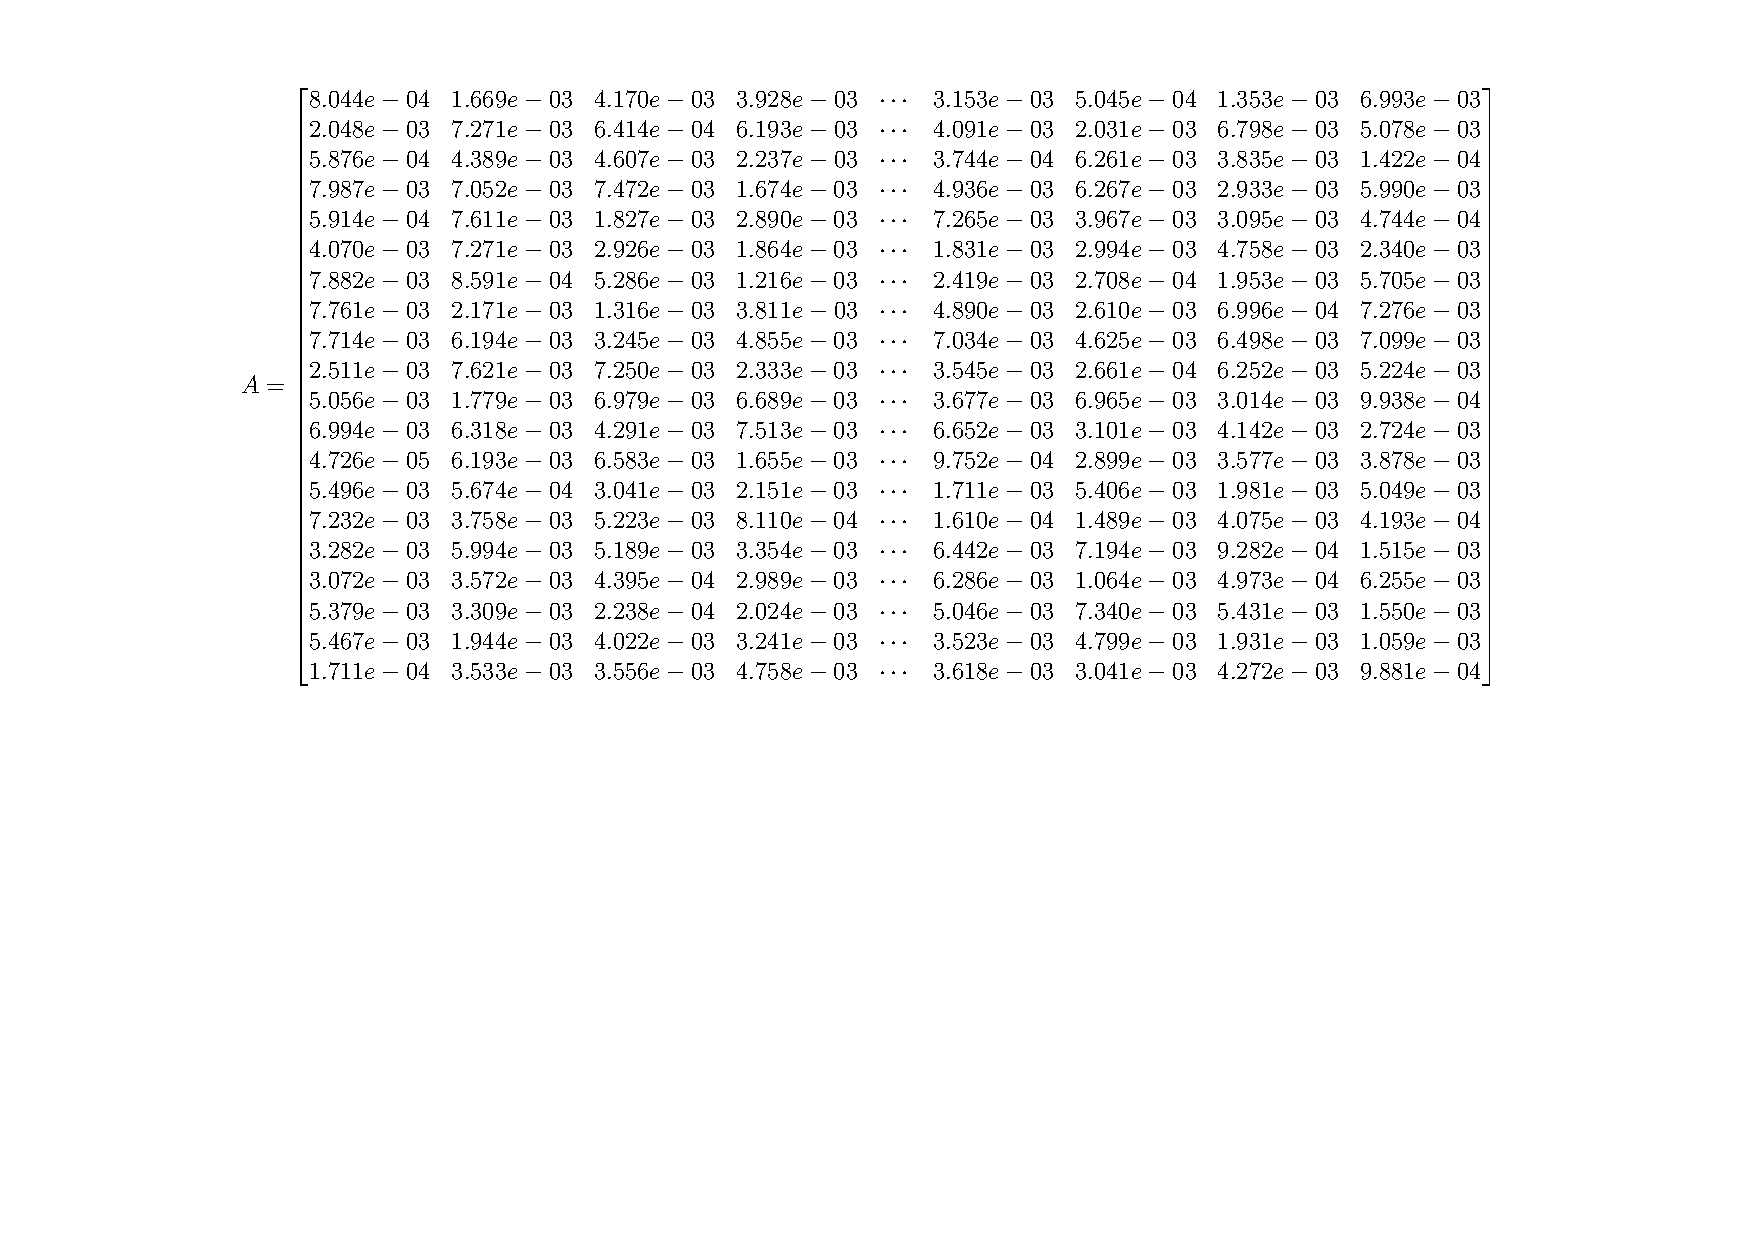
\includegraphics[page=1, trim= 4cm 8.9cm 4cm 1cm ,clip,scale=0.8]{matrix}
\end{center}
\footnote{\href{https://drive.google.com/drive/folders/1IG3zhcmc9r95b-fswaWiVBEHy0orYTWj?usp=sharing}{\underline{click aquí para ver la matriz A completa}}}
\vspace{-1.5cm}
\begin{center}
	\includegraphics[page=2, trim= 4cm 8cm 4cm 1cm ,clip,scale=0.8]{matrix}
\end{center}
\vspace{-1.5cm}
\begin{multicols}{2}
\noindent Donde $a_{ij}$ es el dinero con el que la industria $S_j$ compra productos a la industria $S_i$ para producir \$1 de producto y $d_i$ es la demanda exterior, de una semana, que tiene la industria $S_i$.\\
Nuestro objetivo es hallar el nivel de producción(en dólares) de cada una de las 20 industrias en ese período de una semana para satisfacer exactamente las demandas internas y externas.

\noindent Ahora aplicando el modelo abierto de Leontief, nuestro sistema a resolver es $$(I-A)P=d$$ donde $p_i$ es la producción total(en dólares) de la industria $S_i$.\\
Como este sistema es de $20\times20$ sería ``imposible'' resolverlo manualmente, para resolverlo debemos usar métodos numéricos. En la siguiente tabla se muestra los algoritmos usados para resolver la ecuación, con sus respectivos márgenes de error y su tiempo de demora.\footnote{\href{https://drive.google.com/drive/folders/1F-M1slvs1ibC-nhFcPin_ge0fLCHVb1c?usp=sharing}{\underline{click aquí para ver el código de los métodos}}}
\end{multicols}
\vspace*{1cm}

\begin{center}
	\centering
	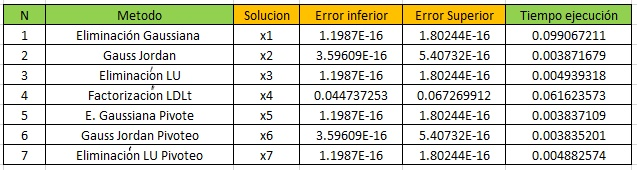
\includegraphics[scale=0.8]{TablasDatos.jpg}
	\\
	Fig1: Datos obtenidos por la computadora empleando métodos numéricos 
\end{center}

\vspace*{1cm}

\begin{center}
	\centering
	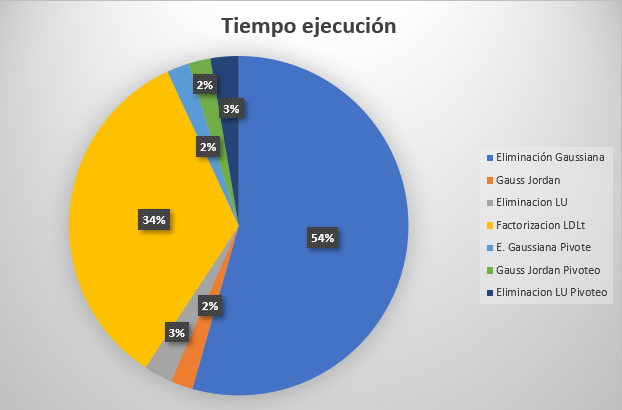
\includegraphics[width=10.5cm,height=7cm]{TiempoEjecucion.PNG}
	\\
	Fig2: Gráfica del tiempo empleado al resolver el sistema
	 
\end{center}

\begin{multicols}{2}
\noindent \textbf{Analizando la Fig 2:} 
Podemos notar que los métodos más lentos en comparación de los demás es Eliminación Gaussiana sin Pivote y LDLt , mientras que la Eliminación Gaussiana con Pivote y Gauss Jordan con Pivote son los dos métodos más rápidos para resolver el problema, ahora tenemos que comparar quien genera una menor cota de error para decir que es el mejor método.\\
\noindent Si bien 5 métodos escogidos son muy rápidos para el problema(matriz de 20 x 20), en la realidad para analizar la economía de un país, nos generan matriz muy grandes(matriz de 500 x 500), es ahí donde se va notar una mayor diferencia en que método es más rápido.
\end{multicols}

\begin{center}
	\centering
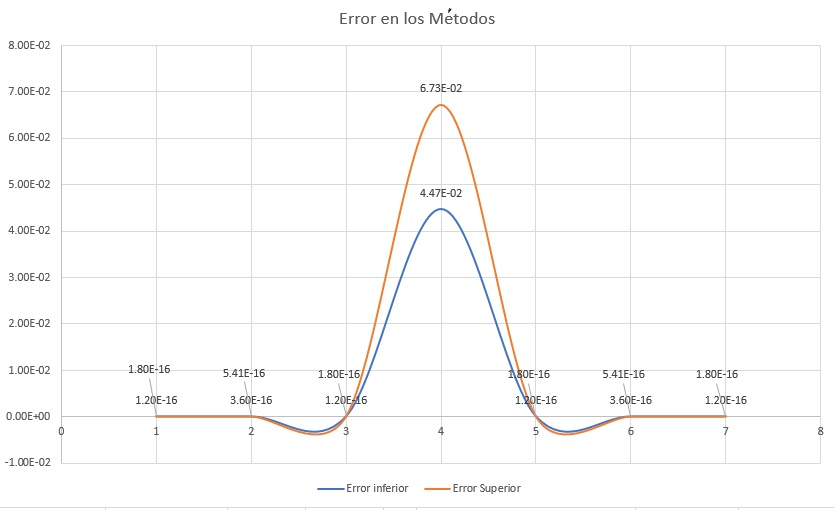
\includegraphics[scale=0.6]{Errorenlosmetodos.jpg}
	
	Fig3: Gráfica de las cotas de error optenidos por cada método, los métodos corresponden con Fig1
\end{center}
\begin{multicols}{2}
\noindent \textbf{Analizando la figura 3}, entre los métodos que tienen una menor cota de error son 1, Eliminación Gaussiana, 3 Eliminación LU, 5 Elimicación Gaussiana con Pivote, 7 Eliminación LU Pivote, viendo que el método más rapido fue Eliminación Gaussiana con Pivote entonces el mejor metodo es Eliminación Gaussiana con Pivote. 
Este algoritmo consiste básicamente en la transformación de una matriz cualquiera en una matriz triangular superior, ya que es mucho más sencillo manipular sistemas de ecuaciones cuya matriz psee dicha característica. Las operaciones elementales en la eliminación de Gauss son tres: multiplicación de una ecuación por una constante que no es cero,sustracción del múltiplo de una ecuación con otra ecuación y finalmente el intercambio de ecuaciones.El primer algoritmo recibe la matriz aumentada conformada por la matriz $a$ y el vector $b$, y transformará el sistema de ecuaciones en un sistema cuya matriz sea triangular superior. Finalmente, para obtener la solución se usa el algoritmo de sustitución inversa. 

\begin{center}
	\centering
	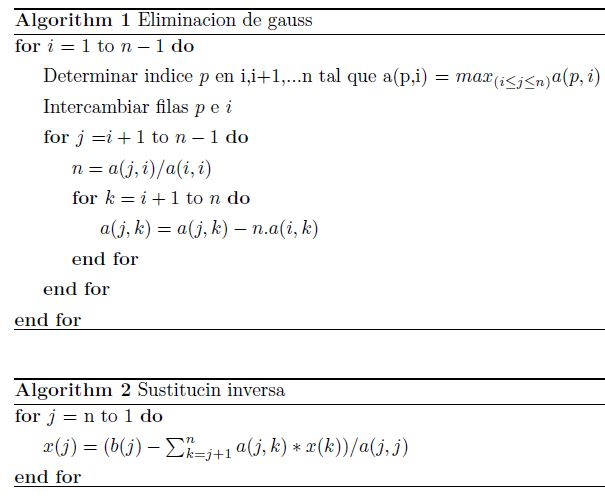
\includegraphics[width=7cm,height=7cm]{algoritmos.jpg}
	\\
	
\end{center}

\noindent Notar que el metodo 4 Factorización LDLt genera una cota de error muy grande, esto se debe a que la matriz del problema, si bien era semidefinida positiva, esta no era simétrica entonces para emplear el método se recurrió a multiplicar por su transpuesta y asi poder emplear el método, este nos genero un error considerable.\\
\end{multicols}


\begin{multicols}{2}
	\noindent Para este problema que consiste en modelar la economía de un país ,usar el método de Factorización LDLt es muy perjudicial, esto podria generar muchas perdidas economicas, generar una mayor inflación y por consecuencia la población seria la más afectada.
	
	\noindent \textbf{Análisis rápido} \\
	De la tabla deducimos que el peor algoritmo para resolver nuestra ecuación es la Factorización $LDL^t$ ya que este es el que tiene mayor rango de error y además es el que más demora en hallar la solución.\\ También observamos que el mejor algoritmo es para resolver nuestro sistema es la eliminación Gaussiana con pivote ya que su rango de error y su tiempo de ejecución son mínimos. Así nuestra mejor solución numérica es $P=X_5$.
	\begin{equation*}
	P=
	\begin{bmatrix}
	14801.59007326\\  
	103454.86190732\\   
	41209.7906775 \\
	102905.97723502\\   
	49404.70709737\\   
	65486.74572585\\
	85458.29205909\\   
	78393.30888981\\   
	39323.16891416\\
	55453.09505371\\   
	83824.60273144\\   
	67779.49104967\\
	45342.78535427\\   
	31478.9479484 \\   
	74892.28078095\\
	56541.07187277\\   
	62008.22170696\\   
	37154.56793729\\
	35097.11057469\\   
	36007.01516564
	\end{bmatrix}
	\end{equation*}
	
%\newpage
%\includegraphics[keyvals]{}
\begin{center}
{\large \bf 4. OBSERVACIONES}
\end{center}
Se observó que para la misma matriz, los márgenes de error y el tiempo de ejecución de cada algoritmo pueden cambiar, y por ende el mejor método depende de la ecuación que se quiera resolver.\\
\begin{center}
{\large \bf 5. CONCLUSIONES}
\end{center}
Para modelar un país se necesita hacer uso de los computadores, ya que estos poseen una enorme cantidad de datos y deben realizar muchos cálculos, realizarlos manualmente sería imposible.\\
El verdadero problema radíca en encontrar el mejor método para resolver el problema.\\
Concluimos que para nuestra ecuación \textbf{el mejor algoritmo es el de eliminación Gaussiana con pivoteo} que nos da como solución $X_5$, así para satisfacer exactamente las demandas internas y externas la industria $S_1$ debe producir  \$$14801,59007326$, la  industria $S_2$ \$$103454,86190732$ y así sucecivamente siguiendo el vector solución.\\
Además concluimos que el \textbf{peor método} empleado para resolver el problema es \textbf{Factorización LDLt}, este nos gerera una cota de error muy grande. Utilizar este método generaría pérdidas de miles de dólares al país.

\begin{center}
{\large \bf Agradecimientos}
\end{center}
Los autores agradecen a las autoridades de la Facultad de Ciencias de la Universidad Nacional de 
Ingenier\'{\i}a por su apoyo.
%\begin{center}
%{\large \bf Apendice: }
%\end{center}

\end{multicols}
\newpage

\begin{center}
 -----------------------------------------------------------------------------
\end{center}
\begin{multicols}{2}
\begin{list}{}{\setlength{\topsep}{0mm}\setlength{\itemsep}{0mm}%
\setlength{\parsep}{0mm}\setlength{\leftmargin}{4mm}}
%
%------------------------------------- References --------------------
\small
\item[1.] Jaan Kiusalaas, \textit{Numerical Methods in Engineering\linebreak with python.} Cambrige University Press \textbf{37} (2010).
\item[2.] L.Héctor Juaréz V., \textit{Análisis Númerico} Universidad Autónoma Metropolitana \textbf{2008} (2010).
\item[3.] W. Kincaid, D. Cheney, \textit{Métodos Númericos y Computación,} sexta edición. Cengage Learning, 300-305.
%---------------------------------------------------------------------
%
\end{list}
\end{multicols}
\end{document}%\grid
